%
% T�TULO DEL CAP�TULO
%
\chapter{Computer Graphics basics
	\label{chapter_3}
}

In this chapter, some concepts in 3D rendering are introduced, paying special attention to the main components of a real time point-based rendering visualizer. We first describe the process that generates the frame-buffer. This means that we have to explain the camera model. We will also depict how we represent points in space by several means that will be introduced in this chapter.

Only a brief description of these concepts is presented, to get more familiarized with Computer Graphics the book \cite{CGPP} is recommended. For point-based rendering techniques the book \cite{pbg} is an essential source.

\section[Rendering]{
	Rendering
}

Traditionally Computer Graphics has been defined as the computer science discipline that is dedicated to synthesizing images algorithmically with computers. Nowadays we can find even more related topics like hyper realistic photography, animation techniques, virtual reality, etc. To generate images from three-dimensional scenes a process called \textbf{render} is used. This set of actions  is in charge of modeling objects and their properties, illumination if needed and the camera that will capture everything.

As has been said before, rendering is the computational process of generating an image from a model. From this definition multiple interpretations are possible, from creating a 3D animation film to a bar chart in a spreadsheet, all of them are equally valid. Although the term is normally used when the model we are using is of a spatial nature and more specifically three-dimensional.

Several classifications of rendering techniques could be made, but for this introduction we will use two of them. On one side, if we use the type or style of the image we want to achieve, we will have:

\begin{itemize}
\item \textbf{Non-photorealistic rendering}, uses other types of effects that render the scene with artistic style, intended to look like a painting or drawing.
\item \textbf{Photorealistic rendering}, tries to be as faithful as possible to reality. This type of render can be subdivided in: 
	\begin{itemize}
	\item \textbf{Physically-based rendering}: Tries to compute an authentic simulation of light transport through the virtual scene and its interaction with materials and objects. The precision of this simulation will depend on the mathematical and physical models chosen.
	\item \textbf{Faked}: Utilizes algorithmic tricks, not trying to pretend an ad-hoc simulation of light, usually to reduce render times.  
	\end{itemize}
\end{itemize}

\begin{figure}[h]
	\centering
	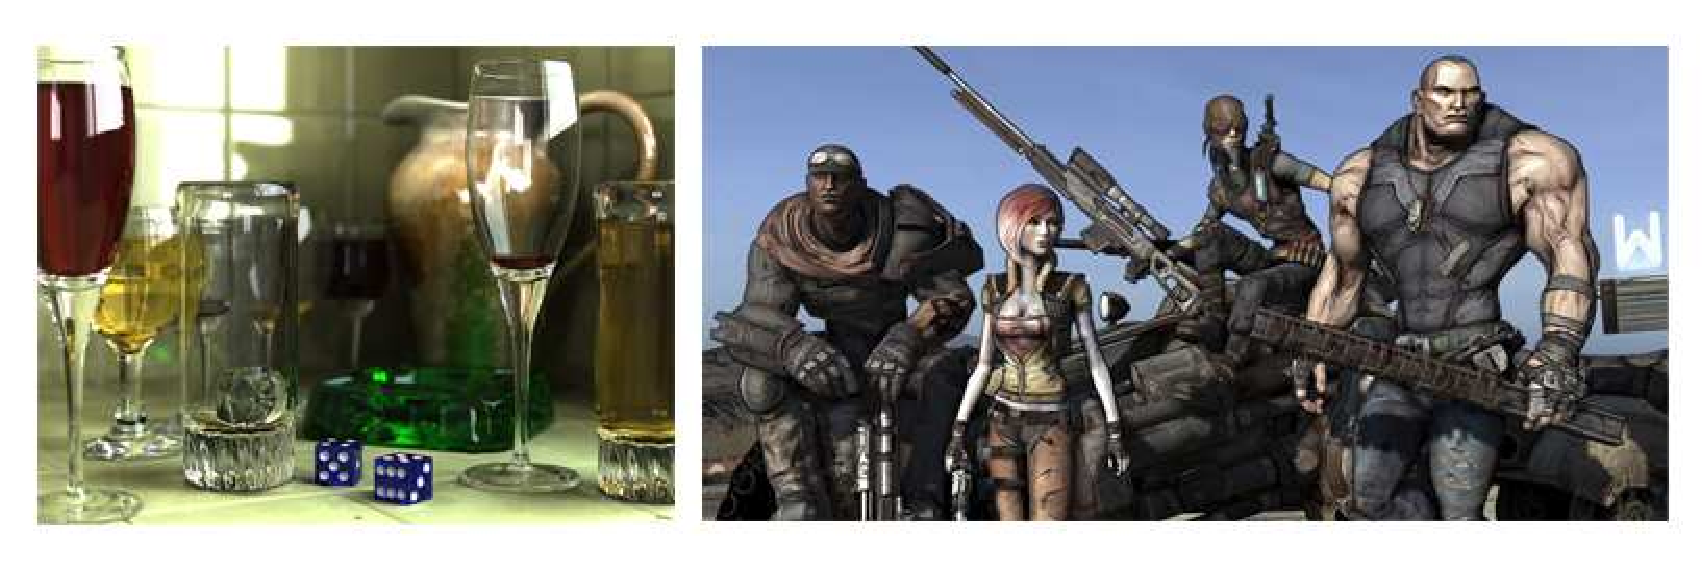
\includegraphics[scale=0.5]{figures/photo_comp.pdf}
	\caption[Rendering types comparison]{
		A photorealistic render on the left, versus a non-photorealistic render on the right.
	}
	\label{photo_comp}
\end{figure}

On the other side, if we compare the interaction capabilities of the rendering application with the user, we can divide rendering techniques in: 

\begin{itemize}
\item \textbf{Offline rendering}: Where the process that generates the image is too slow to respond instantaneously to the user interactions. A time scale of seconds and up to several days can be considered ``slow''. This happens for example when generating photograms for a movie.
\item \textbf{Online rendering}: Where processing time would be short enough to respond to user interactions so that the user has the sensation of continuity. A time scale of miliseconds would be needed to achieve this effect. Normally it is measured in \emph{frames per second} (FPS). A good example of this technique are videogames. 
\end{itemize}

Almost everything in this document will be devoted to non-photorealistic real-time rendering techniques, since ToView is aimed as way for the user to interact in real-time with massive point clouds.

For more information about real-time rendering please consult \cite{realtime}.

\subsection[Rendering process]{Rendering process}

There are several techniques for generating images from a model. All of them start with a camera position, the geometry of the objects is projected in that direction one way or another, calculating the color of each resulting pixel. The two families of techniques are the ones based on \emph{scanline rendering}, where lists of geometry are traversed with horizontal scan lines. Intermediate calculations determine what object is closer to the camera, how do the lights in the scene affect the objects, etc.

Since we require real-time rendering, we will take advantage of the power of the GPU. The GPU \textit{pipeline} is the process implemented in hardware to create images from the scene information in a highly efficient way. It is comprised of several stages were several lineal algebra operations that account for the position, rotation and scaling of the point of view, objects and lights; to finally determine the color of the pixel drawn to the screen. 

A GPU can be used to process graphical data using two APIs\footnote{\textit{Application Programming Interface}}:

\begin{itemize}
\item \textbf{DirectX}: Microsoft's propietary API, only useful in Windows systems. 
\item \textbf{OpenGL}: Standard and multiplatform, this were the main reasons why it was the chosen API for this project. 
\end{itemize}

\begin{figure}[h]
	\centering
	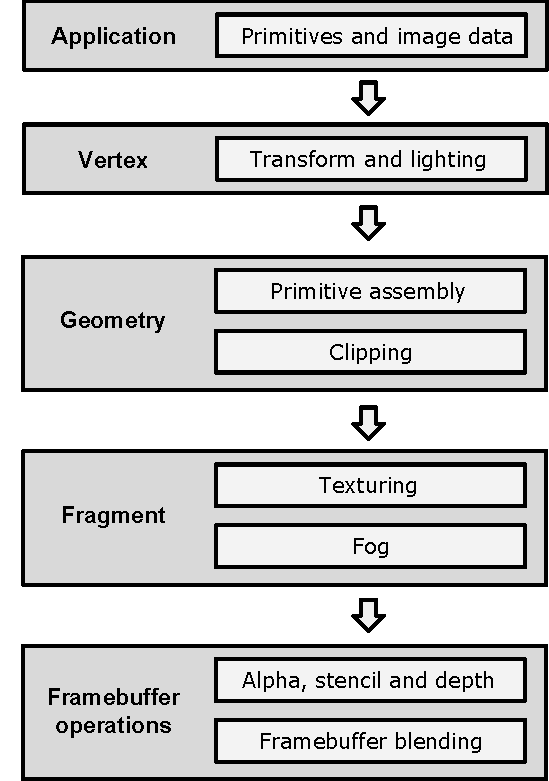
\includegraphics[scale=0.6]{figures/ogl_pipe.pdf}
	\caption[OpenGL pipeline]{
		The OpenGL pipeline.
	}
	\label{opengl_pipe}
\end{figure}

In modern GPUs, some of the stages of the pipeline can be modified using small programs written in GLSL\footnote{\textit{GL Shading Language}} called shaders. In \figurename~\ref{opengl_pipe} the simplified pipeline of a modern version of OpenGL can be observed. In it the vertex, geometry and fragment stages are programmable. The \textit{frame-buffer}\footnote{The portion of memory (buffer) reserved to maintain temporally an image (frame) awaiting to be sent to the monitor.} will be the final image that will be shown onscreen. 

Although there are some constraints in the form of number of instructions and control structures, shaders started a revolution in real-time rendering. Sometimes even allowing to create images almost as realistic as offline rendering.  

\subsection[Models]{
	Models
}

Modeling describes the process of forming the shape of a virtual object in a computer. There are several types of models (see \figurename~\ref{model_comp}):

\begin{itemize}
\item \textbf{Polygon-based}: Describe the surface of an object as a set of polygons. Triangles are the most commonly used polygons, since they are flat and trivially convex. Most of the existing graphics hardware is optimized for this primitive.
\item \textbf{Voxel-based}: Divides space in a regular 3D grid where the \emph{voxel} is the smallest unit of volume. Each cell is either filled or not and depending on that the pixels are shaded. Memory increases as precision is augmented. 
\item \textbf{Point-based}: Objects are represented by point samples of their surface, that is why they are usually called \emph{splats}. Each point has a position and some information about the surface that it belongs to. Compared to the traditional triangle-based approach, this primitive needs its own rendering techniques and its own pipeline, since different challenges must be faced. This is our case study and because of that, this primitive will be further explained in Section~\ref{splats_and_points}.
\end{itemize}

\begin{figure}[h]
	\centering
	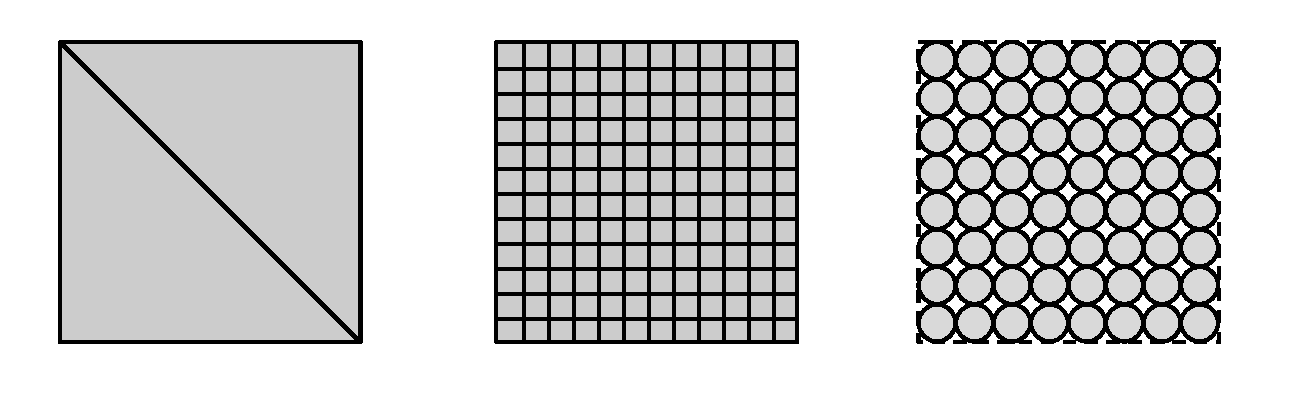
\includegraphics[scale=0.6]{figures/model_comp.pdf}
	\caption[Model types comparison]{
		From left to right; a polygon-based, a voxel-based and a point-based model of a plane (2D representation).
	}
	\label{model_comp}
\end{figure}

%
% SECCION - T�tulo de la secci�n
%
\section[Splats]{\label{splats_and_points}
	Splats and points
}

A point cloud is a set of vertices or points in a three-dimensional coordinate system. These vertices are usually positioned in 3D space and have a set of coordinates $(x,y,z)$. These sets of points normally are representative of the external surface of an object. 

\begin{figure}[h]
	\centering
	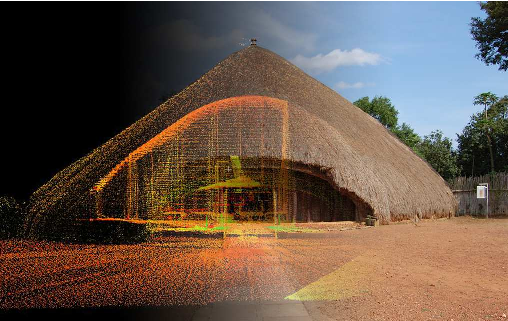
\includegraphics[scale=1]{figures/point_cloud.pdf}
	\caption[Point cloud]{
		Photo overlaid atop laser scan data from a project held in early 2009 at Kasubi Tombs.
	}
	\label{point_cloud}
\end{figure}

Point clouds are normally created by 3D scanners, these devices capture automatically a large number of points on the surface of an object (see \figurename~\ref{point_cloud}), and yield a point cloud dataset as a result. 

The points from the range data represent a surface, but a point is zero-dimensional; this means that it does not have volume, area, length or any other higher dimensional equivalent. Usually point clouds are not directly usable in most 3D applications because of this reason. That is why we need splats (surface elements), that describe the surface in a small neighborhood. 

At this point we need to choose how the surface will be represented by the point. In our project we will represent the splat as a disc. 

\begin{figure}[h]
	\centering
	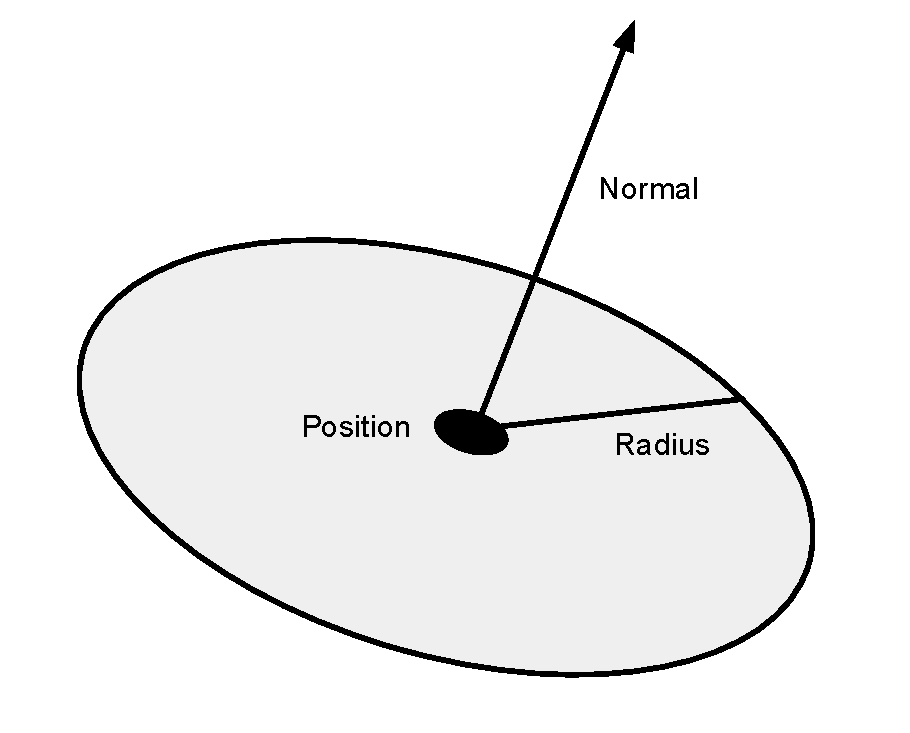
\includegraphics[scale=0.4]{figures/surf_disc.pdf}
	\caption[Disc approach]{
		Visual representation of the splat as a disc.
	}
	\label{surf_disc}
\end{figure}

If on the other hand we choose to represent the splat as a disc, the splats can have have the following parameters (see \figurename~\ref{surf_disc}):

\begin{description}
  \item [Position:] \emph{x}, \emph{y} and \emph{z} coordinates in world space.
  \item [Normal:] A vector that represents the surface normal of the splat. It can be provided or the engine can estimate it.
  \item [Radius:] This will be the radius of the sphere that will represent the splat. The engine will also be capable of calculating the radius automatically.
  \item [Color:] The splat color in RGB parameters if we are going to use the lighting from the scanned data.
  \item [Other properties:] Intensity, reflectivity, temperature, etc.
\end{description}

\section[Transformations]{
	3D Euclidean space and transformations
}

In 3D computer graphics we normally work with a three-dimensional space of Euclidean geometry, the term ``Euclidean'' is used to distinguish between these spaces and the curved spaces of non-Euclidean geometry. The most common types of operations in Euclidean geometry can be represented with a transformation matrix if homogeneus coordinates are used. Because of this a transformation \textbf{T} can be used for several purposes. 

Using basic linear algebra concepts, a $4\times4$ matrix can be used to express the linear transformation of a point or vector. A transformation will then be represented by the elements of the $4\times4$ matrix. They can also be used to perform some transformations that are non-linear on an Euclidean space. For this reason transformation matrices are widely used in computer graphics.

Generally a transformation is a mapping from points to points or vectors to vectors \cite{PBRT}, for example: \begin{equation}p' = \textbf{T}(p) \;\;\;\;\; v' = \textbf{T}(v)\end{equation} 

To transform the points or vectors we just have to perform the appropriate matrix multiplications. This also allows the composition of transformations, we just have to multiply the transformation matrices. 

Most commonly used transformations are:

\begin{itemize}
\item \textbf{Rotation}, will rotate a point or a vector by a given angle either around an arbitrary axis or the $x$, $y$ or $z$ axis.
\item \textbf{Scaling}, takes a point or a vector and will scale its $x$, $y$ and $z$ components by a factor.
\item \textbf{Translation}, only affects points and will translate coordinates $x$, $y$ and $z$ a set amount.
\item \textbf{Model}, this matrix is useful for transforming the model locally. It is comprised of a set of rotation, scaling and translation matrices. When we apply this matrix to all the points, we will have them in world coordinates.  
\item \textbf{View}, initially the camera is placed in the origin of world space. To be able to move around the world this transformation is used. This matrix is also called \textit{look-at}. After this transformation is applied, we will have the points in camera coordinates.
\item \textbf{Projection}, since a 3D scene has to be projected onto the screen as a 2D image, we need another process that converts the points from camera coordinates to homogeneous coordinates so that they can be projected onscreen. 
\end{itemize}

Usually the composition of the model, view and projection matrices is called \textit{MVP} and is applied to every point that we want to draw.

To illustrate how the transformations are represented by a $4\times4$ matrix, equation~\ref{eq_trans} shows the generic transformation matrix for a translation: \begin{equation}\label{eq_trans}\textbf{T}(\Delta x,\Delta y,\Delta z) = \begin{pmatrix}
 1& 0 & 0 & \Delta x\\ 
 0& 1 & 0 & \Delta y\\ 
 0& 0 & 1 & \Delta z\\ 
 0& 0 &0  & 0
\end{pmatrix}\end{equation}

This transformation is applied to a point $P=(x,y,z)$ in the following way: \begin{equation}\begin{pmatrix}
 1& 0 & 0 & \Delta x\\ 
 0& 1 & 0 & \Delta y\\ 
 0& 0 & 1 & \Delta z\\ 
 0& 0 & 0 & 0
\end{pmatrix} \begin{pmatrix}
x\\
y\\
z\\ 
1
\end{pmatrix} = \begin{pmatrix}
x+\Delta x\\
y+\Delta y\\
z+\Delta z\\ 
1
\end{pmatrix}\end{equation}

\section[Camera model]{\label{camera_model}
	Camera model
}

Almost everyone nowadays has used a camera and knows its basic purpose: you want to record an image of the world (usually pressing a button) and the image is then recorded on a film. One of the simplest  cameras in the real world is the \emph{pinhole camera}. Pinhole cameras use a light tight space with a hole at one end. When this hole is uncovered light enters through the hole and reaches a piece of photographic paper on the other end of the box (see \figurename~\ref{pinhole}). In this day and age, cameras are more complex than this simple camera model, but this is a good starting point to explain how our simulation works.

\begin{figure}[h]
	\centering
	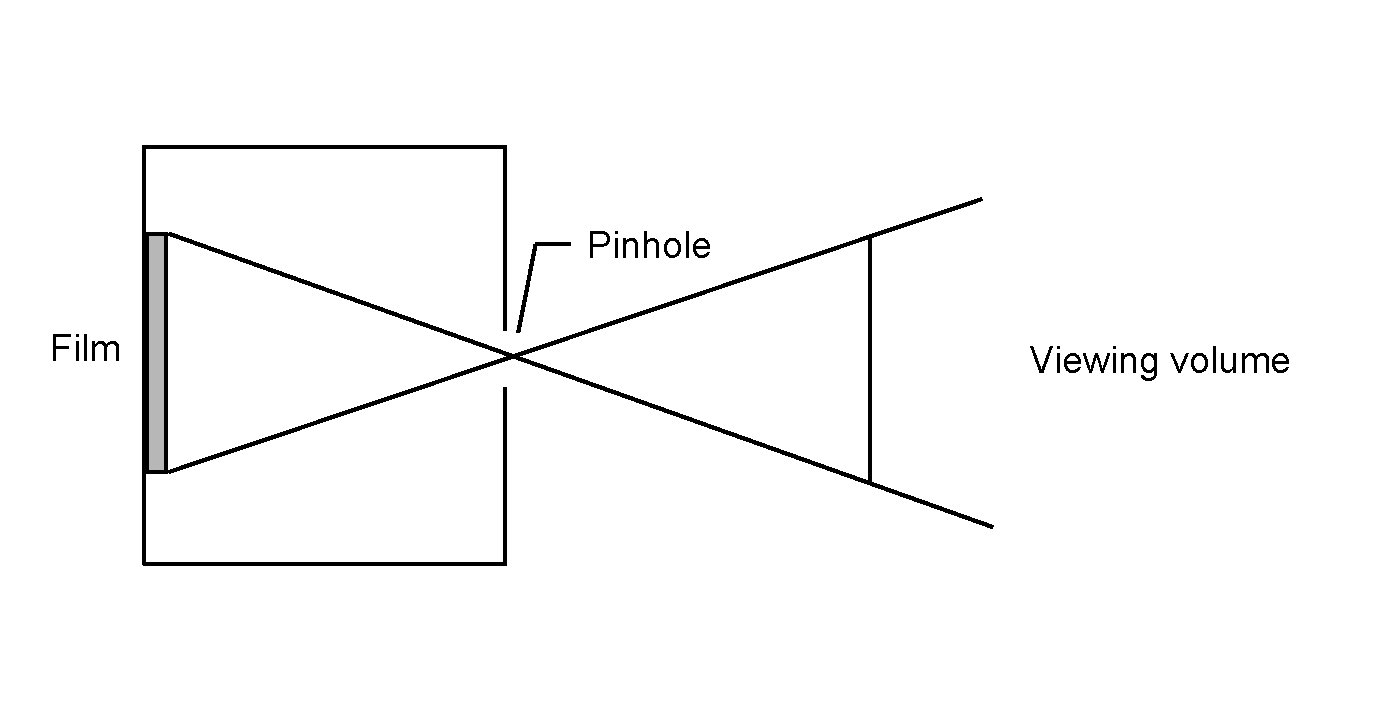
\includegraphics[scale=0.5]{figures/pinhole.pdf}
	\caption[Pinhole camera]{
		Diagram explaining how a pinhole camera works.
	}
	\label{pinhole}
\end{figure}

The most important function of the camera is defining the part of the scene that will be recorded on the photographic film. Connecting the pinhole to the edges of the film creates a double pyramid that extends into the scene. Objects that are not inside this pyramid will not be imaged on the film. As cameras are now more complex, we will refer to the region that can be imaged as \emph{viewing volume}. 

If we were to use the pinhole as the film, the viewing volume would not change. When the film or image is infront of the pinhole, the pinhole is frequently referred to as the \emph{eye}. In our simulated camera where the film is infront of the eye, we will display the amount of light traveling from the image plane to the eye. Several tests will be performed by OpenGL depending on the type of camera to check which points can be seen and have to be represented in the frame-buffer. 

The camera model used in this project supports several settings. First we explain how this settings affect the camera model, after we detail how the camera model interacts with the ray tracing process. Readers can consult \cite{PBRT} if they want to delve deeper in the topic.

\subsection[Parameters]{Camera parameters}

The first parameter that the camera model supports is \textbf{camera position}. This parameter states where the camera will be positioned in world space coordinates (\emph{x,y,z}).

Next supported parameter is the \textbf{camera orientation}. This parameter is a point in the world at which the camera is looking at.

\begin{figure}[h]
	\centering
	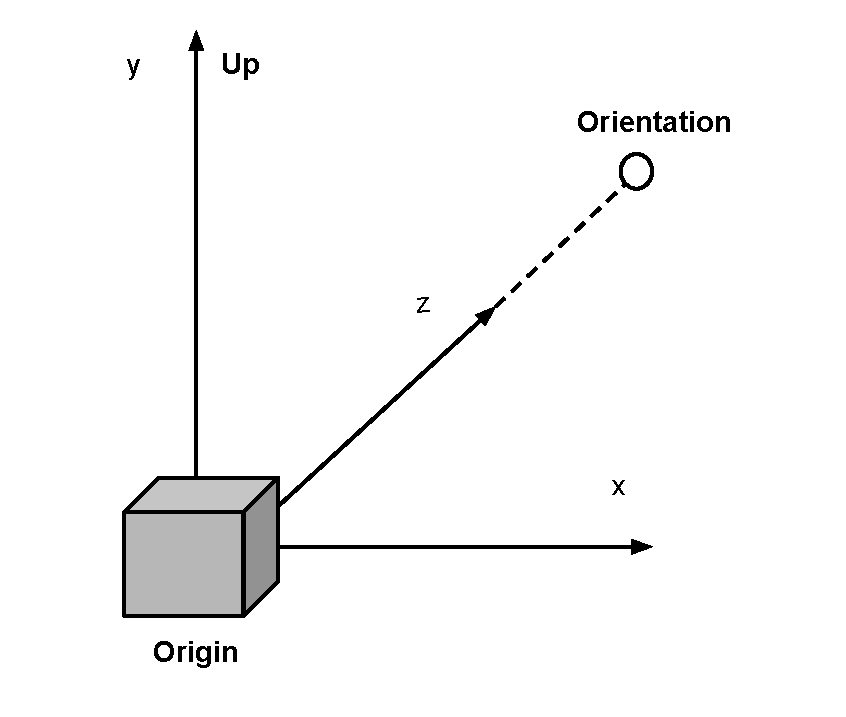
\includegraphics[scale=0.55]{figures/cam_ori.pdf}
	\caption[Camera orientation]{
		Diagram explaining the camera coordinates.
	}
	\label{cam_ori}
\end{figure}

We also need to know how to orient the camera along the viewing direction implied by the first two parameters. The parameter \textbf{camera up vector} gives us that orientation. 

We can see how this parameters are organized in camera space in \figurename~\ref{cam_ori}.

Other important parameters in a camera model are the clipping planes. \textbf{Hither} dictates where the near clipping plane of the camera is located and \textbf{yon} indicates where the far clipping plane is situated as we can see in \figurename~\ref{hither_yon}. The camera's clipping planes give us the range of space along the \emph{z} axis that will be visible in images. Objects that are in front of the hither plane or beyond the yon plane will not be visible. 
\begin{figure}[h]
	\centering
	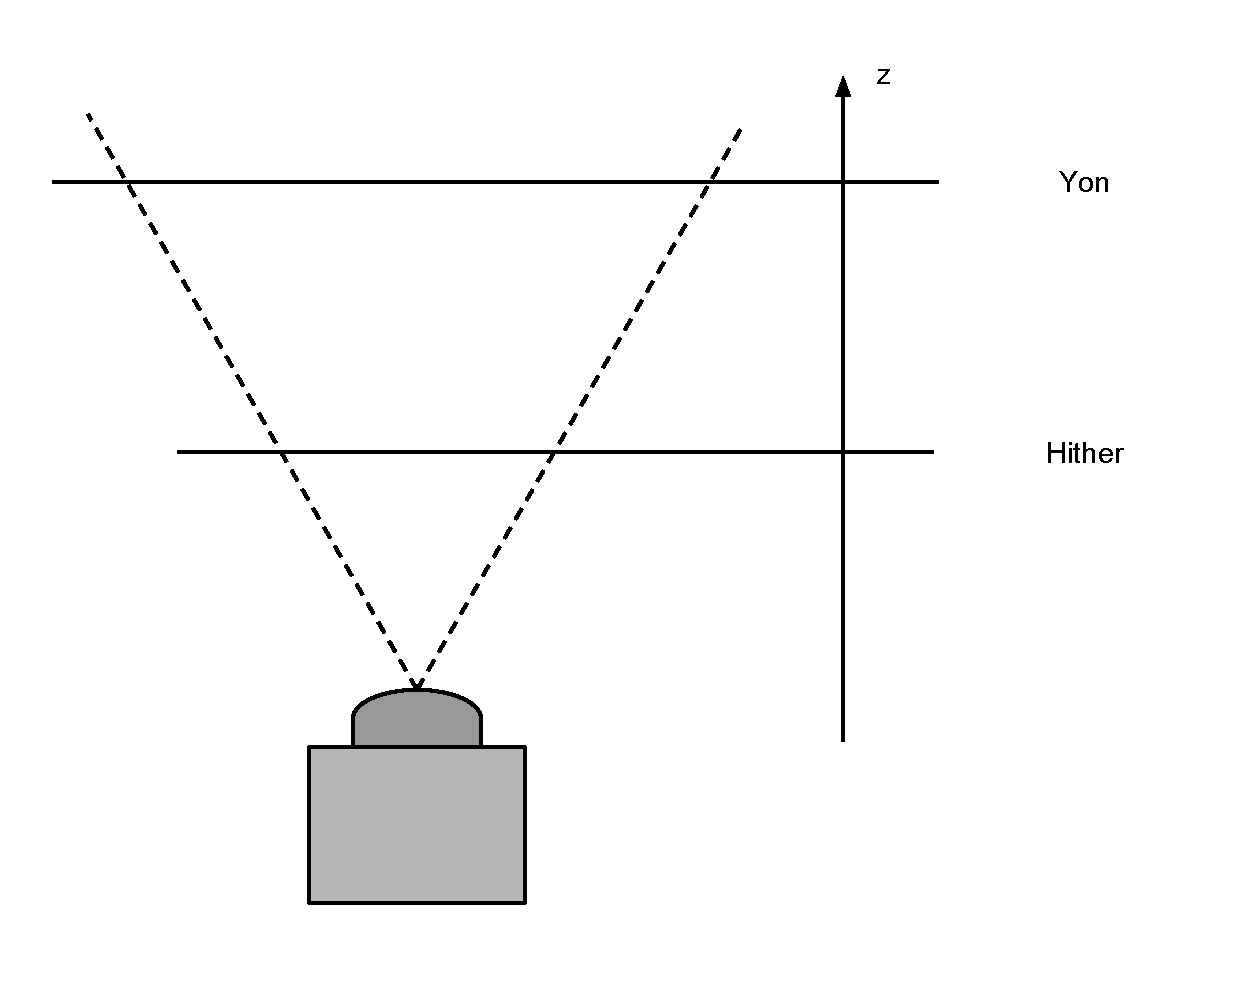
\includegraphics[scale=0.45]{figures/hither_yon.pdf}
	\caption[Hither and Yon]{
		Representation of hither and yon planes.
	}
	\label{hither_yon}
\end{figure}

The last parameter that the camera supports is the \textbf{field of view}. The angle of view describes the angular extent of the scene captured by the camera horizontally and vertically. 

The clipping planes and the angles of view define the viewing volume in our model, also known as the \emph{viewig frustum} (see \figurename~\ref{frustum}).

The user also has the option to use a \textbf{perspective} or \textbf{orthographic} camera depending on what his needs are. An architect for example may prefer an orthographic camera, while a normal user may use a perspective camera that will yield a more natural image as result (see \figurename~\ref{pers_ort}). 

\begin{figure}[h]
	\centering
	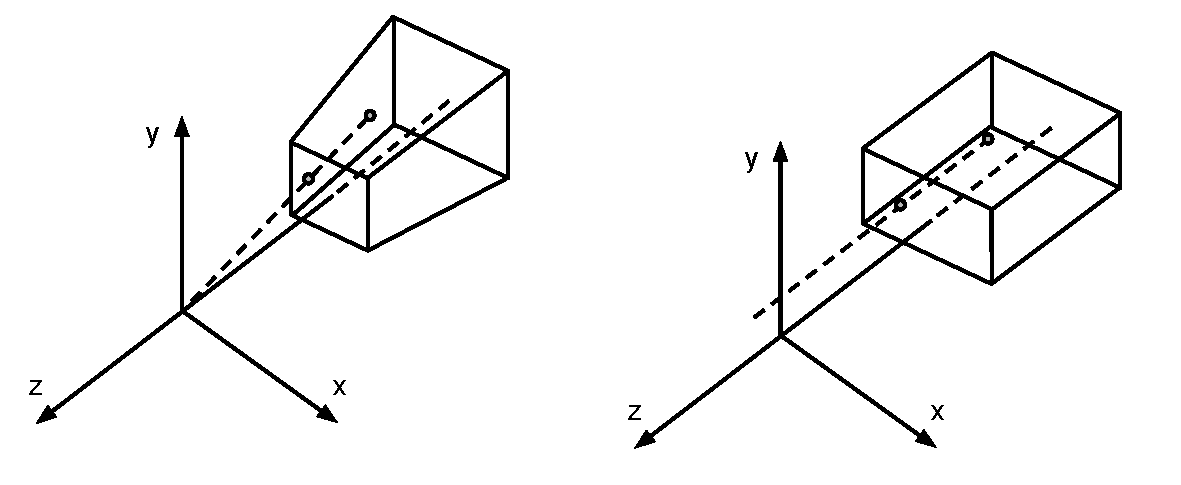
\includegraphics[scale=0.6]{figures/pers_ort.pdf}
	\caption[Perspective and orthographic camera comparison]{
		Representation of the difference between a perspective (left) and orthographic camera (right).
	}
	\label{pers_ort}
\end{figure}

Orthographic projection is more commonly used in engineering because dimensions are communicated unambiguously, if there is a one unit length line anywhere in the scene; it will appear the same length everywhere. Also every line that is parallel in the scene will be parallel in reality. With perspective projection, lines of identical real-world length will appear different due to \textit{foreshortening}\footnote{Objects becoming smaller on the image plane as they get further away.}. This is why it will be difficult to judge relative dimensions when objects are far away.

Another option that is available is using a \textbf{FPS}\footnote{First-Person Camera} or an \textbf{orbital} camera. On one hand with a first person camera the user can walk freely just like if he was inside the scene, forward, back, left, right, etc. On the other hand with an orbital camera the user sets a center point and then orbits around said point.     

\subsection[Inner workings]{Camera inner workings}

Once we have the camera parameters we need to place the camera in the scene, we will use a \emph{look-at} transformation for this purpose. Using the look-at transformation as view matrix will give us a transformation between world and camera coordinates as mentioned before. The matrix is constructed using the position ($p$), orientation ($o$) and up ($u$) vector. 

First, a forward vector $f$ is constructed:

\begin{equation}f = \frac{p - o}{\left \| p - o \right \|}\end{equation}

Next, the right vector $r$ is constructed:

\begin{equation}r = f \times u\end{equation}

After, a new up vector $u'$ is calculated in the camera reference:

\begin{equation}u' = r \times f\end{equation}

With these, a rotation matrix can be constructed representing a reorientation into the newly created orthonormal basis:

\begin{equation}R = \begin{bmatrix}
r_{x} & u'_{x} & f_{x} & 0\\ 
r_{y} & u'_{y} & f_{y} & 0\\ 
r_{z} & u'_{z} & f_{z} & 0\\ 
0 & 0 & 0 & 1
\end{bmatrix}\end{equation}

Finally, to transform objects into the camera's frame; not only everything has to be oriented correctly, it also has to be translated from the origin to the position of the camera. This is achieved by concatenating the rotation matrix $R$ with the corresponding translation matrix:

\begin{equation}\label{view}V = \begin{bmatrix}
r_{x} & u'_{x} & f_{x} & -p_{x}\\ 
r_{y} & u'_{y} & f_{y} & -p_{y}\\ 
r_{z} & u'_{z} & f_{z} & -p_{z}\\ 
0 & 0 & 0 & 1
\end{bmatrix}\end{equation}

Equation \ref{view} is the resulting  look-at matrix \textbf{\textit{V}} that will be used to transform the points from world space to camera space.

The next step will depend on the type of camera that the user will choose, either orthogonal or perspective. In light of this a projection matrix will be chosen reflecting the choice. 

If a perspective camera is chosen, we have to take into account the foreshortening effect we mentioned before. This projection does not preserve distances or angles, and parallel lines no longer remain parallel. \emph{x} and \emph{y} are not left unchanged, they are modified according to the corresponding \textit{z} value, that dictates how close to the camera the point is (see \figurename~\ref{pers_ort}). To achieve this effect, a perspective projection matrix will be used. A commonly used matrix is the \textit{frustum matrix}. In it the homogeneous space takes the shape of a truncated pyramid. The parameters used to construct this matrix are left ($l$), right ($r$), top ($t$), bottom ($b$), near plane ($n$) and far plane ($f$) of the frustum. 

$t$ is obtained in the following way using the camera parameters field of view ($fov$) and hither ($n$):

\begin{equation}t = n \cdot tan(fov / 2) \end{equation} 

Next, $r$ is obtained using the width ($w$) and height ($h$) of the window:

\begin{equation}r = t \cdot w / h \end{equation}   

Since the frustum is symmetric, $l$ and $b$ will be the same as $r$ and $t$ but with the opposite sign. Once we have all of the parameters we can construct the perspective or orthographic matrices:

\begin{equation}\label{pers}P = \begin{bmatrix}
\frac{2 \cdot n}{r - l} & 0 & \frac{r + l}{r - l} & 0\\ 
0 & \frac{2 \cdot n}{t - b} & \frac{t + b}{t - b} & 0\\ 
0 & 0 & \frac{n + f}{n - f} & \frac{2 \cdot n \cdot f}{n - f}\\ 
0 & 0 & -1 & 0
\end{bmatrix}\end{equation}

In contrast, if a orthographic camera is required, a somewhat simpler orthographic projection matrix can be used. Points will be projected to the near viewing plane. This type of transformation does not give the effect of foreshortening, it keeps lines parallel and preserves relative distance between objects. This transformation leaves \emph{x} and \emph{y} coordinates unchanged, but maps \emph{z} values at the hither plane to 0 and \emph{z} values at the yon plane to 1 (see \figurename~\ref{pers_ort}). The parameters used to construct this matrix are also left ($l$), right ($r$), top ($t$), bottom ($b$), near plane ($n$) and far plane ($f$) of the frustum:

\begin{equation}\label{ortho}P = \begin{bmatrix}
\frac{2}{r - l} & 0 & 0 &  \frac{l + r}{l - r}\\ 
0 & \frac{2}{t - b} & 0 & \frac{b + t}{b - t}\\ 
0 & 0 & \frac{2}{n - f} & \frac{n + f}{f - n}\\ 
0 & 0 & 0 & 1
\end{bmatrix}\end{equation}

One of these two matrices (\ref{pers} or \ref{ortho}) will represent the projection matrix \textbf{\textit{P}}.

The composition of these matrices will yield the MVP matrix \cite{OGLSB}. This is the mathematical expression used for transforming each point:

\begin{equation}\begin{split}v' & = \textbf{\textit{P}}\cdot \textbf{\textit{V}} \cdot \textbf{\textit{M}} \cdot v \\ & = \textbf{\textit{MVP}} \cdot v\end{split}\end{equation}    

Once we have the MVP matrix, we can perform \emph{frustum culling}. The visualizer selects the only the points that fall inside the \emph{viewing frustum} (see \figurename~\ref{frustum}). This is a essential process to achieve the necessary performance to be able to render the point clouds in real-time. The viewing frustum is the region of space that will appear in the images generated by the visualizer. This process of eliminating objects that are outside the viewing frustum is called \emph{viewing frustum culling}.

Once we have the adequate coordinates we just have to map them to screen space depending on the resolution of the render. If two points are mapped to the same pixel we have to see which one is closer in the \emph{z} axis, because that will be the point that the pixel is going to represent.

\begin{figure}[h]
	\centering
	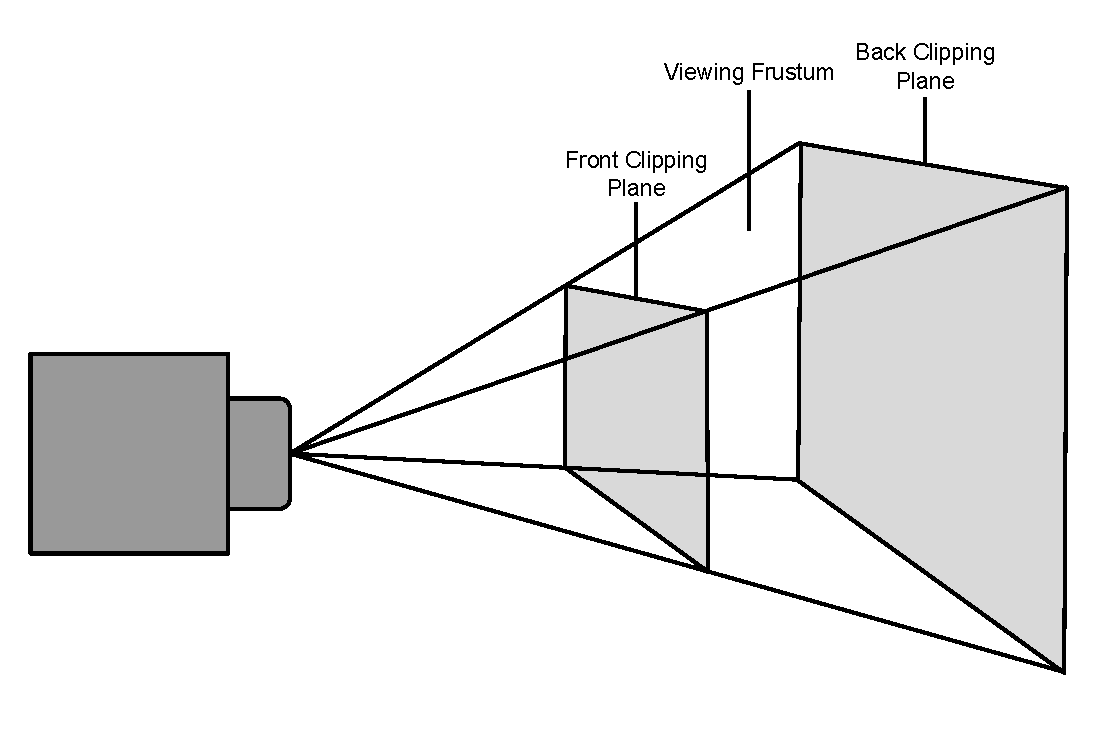
\includegraphics[scale=0.55]{figures/frustum.pdf}
	\caption[Viewing frustum]{
		Diagram showing the viewing frustum.
	}
	\label{frustum}
\end{figure}

These computations are costly when the scenes are big and to simplify the culling process we need an acceleration structure. These structures reject chunks of the scene that are not inside the frustum. In our project we have chosen to use a multi-resolution \emph{k-d tree}.

\begin{figure}[h]
	\centering
	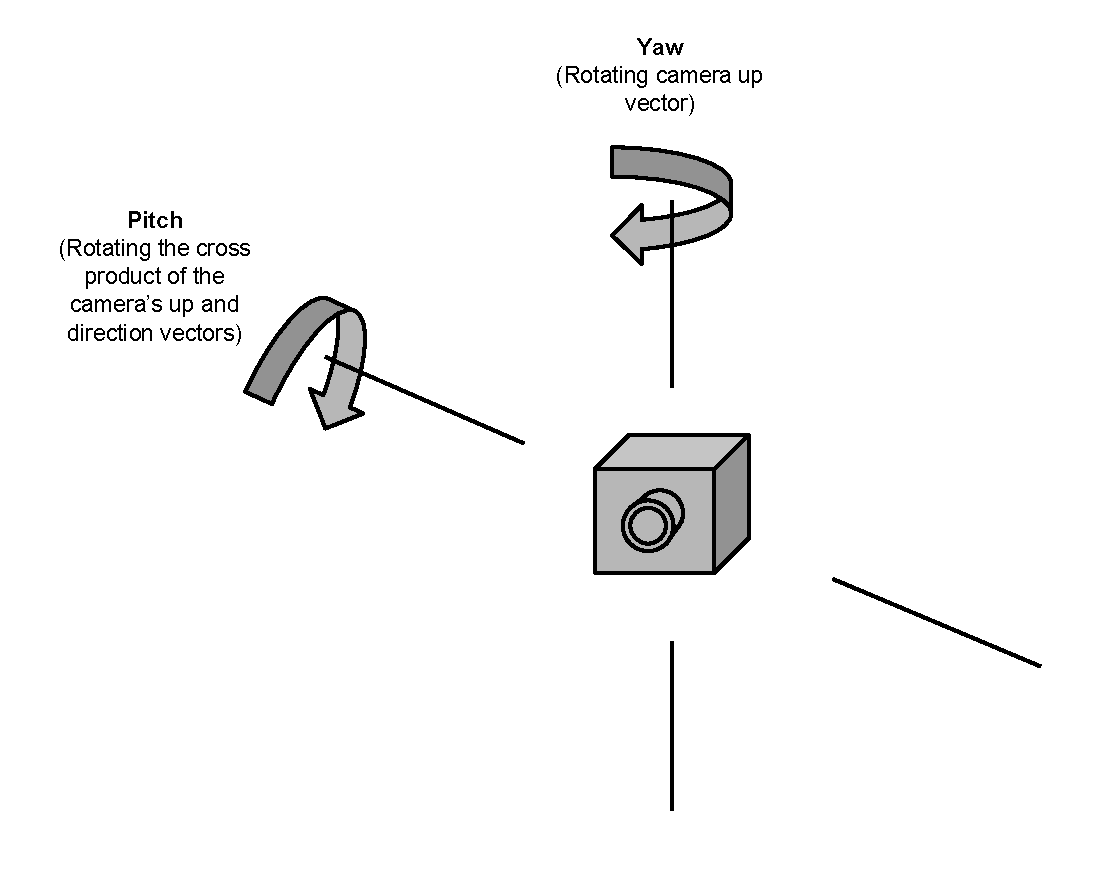
\includegraphics[scale=0.5]{figures/cam_rotation.pdf}
	\caption[FPS camera rotation]{
		Diagram showing the rotation in a first-person camera.
	}
	\label{FPS_rot}
\end{figure}

This is the course of action followed to create one frame, but since the visualizer is interactive, we have to repeat this process several times per second. Furthermore, we have to take into account how the user wants to move. If the FPS camera option is chosen, we start in a certain position and then we will be able to move forward, backward, left and right just as we would be able to do if we were walking around the scene in reality. The user will also be able to look around with complete freedom (see \figurename~\ref{FPS_rot}). \textit{Yaw} allows the user to look left and right and \textit{pitch} up and down.   

When the orbital camera is used, instead of freely walking around, we orbit around a center point (see \figurename~\ref{orb_rot}). The rotation in this instance is represented by a number of rotation degrees ($\alpha$ and $\beta$) around the $x$ and $y$ axes of a coordinate system centered in the interest point. Instead of moving the camera, we move the point of interest, that will be followed by the camera.  

\begin{figure}[h]
	\centering
	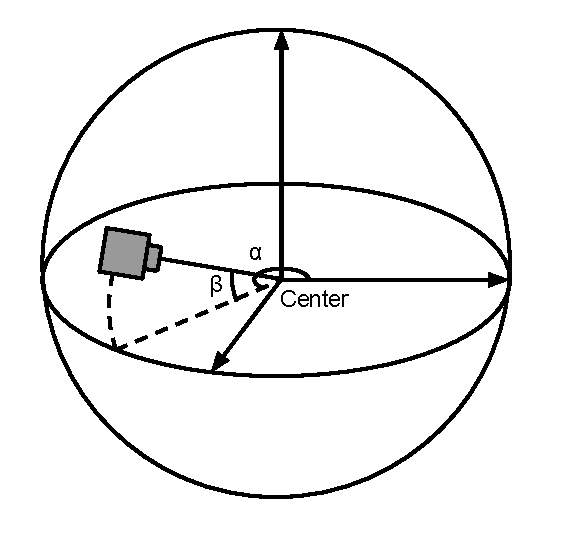
\includegraphics[scale=0.8]{figures/orb_rot.pdf}
	\caption[Orbital camera rotation]{
		Diagram showing the rotation in a orbital camera.
	}
	\label{orb_rot}
\end{figure}







